\providecommand{\mainpath}{../..}
\documentclass[\mainpath/main/main.tex]{subfiles}


\begin{document}

% Title version 1
% \def\localalign{\centering}
%
% \titleformat{\chapter}[display]
% {\normalfont}
% {
%     \localalign{\fontsize{60}{70}\selectfont\thechapter}
% }
% {0.15cm}
% {\color{black}\fontsize{30}{40}\normalfont\localalign #1}
%
% \titlespacing*{\chapter}{0pt}{2ex}{10ex}

% Title version 2
\titleformat{\chapter}[display]
{\normalfont}
{
    \raggedleft\Large\textbf{\textsc{Chapter}}\enspace{\fontsize{50}{60}\selectfont\thechapter}\\
    \rule{\textwidth}{3.0pt}
}
{0.15cm}
{\color{black}\fontsize{30}{36}\normalfont\raggedleft #1}

\titlespacing*{\chapter}{0pt}{2ex}{8ex}


\chapter[Introduction]{Introduction}
\label{ch:introduction}
\usingnamespace{introduction}


%% =============================================================================
%% CHAPTER APHORISM
\aphorismMOD[Stranger in a Strange Land]%
{``Posso dire solo una cosa: Aguuu''}%
{Autore della frase}%
{0.4\linewidth}
%% =============================================================================

\noindent Insert aim and motivation of the work. Fare introduzione dicendo che ci sono tante piattaforme di quantum computer... perché i rydberg atoms? Il problema è la bassa fidelity dei gate con rydberg atoms. Cerchiamo di studiare come vari effetti influiscono sulla fidelity. Per fare ciò utilizziamo quantum control per trovare impusli ideali. Parlare del quantum control.

Parlare dell'esperimento qryd Ref.~\cite{Aaronson2011}


\begin{figure}[h!]
\centering
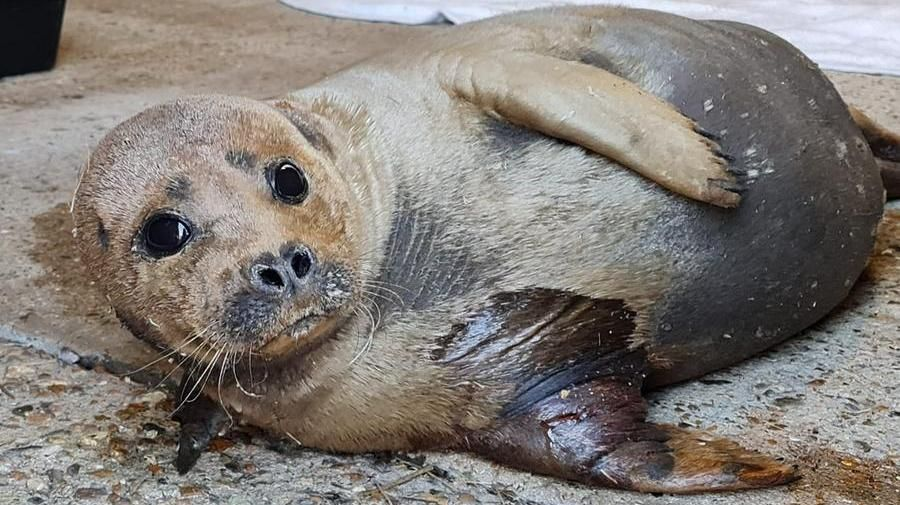
\includegraphics[width=1\textwidth]{\mainpath/chapters/introduction/figures/prova.jpeg}
\caption[Short caption]{\label{fig:} Questa è la prima figura che inserisco.}
\id{fig:prova}
\end{figure}

Nella figura \idref{fig:prova}

In \idref{sec:sezione_uno}, we talk about ....

\section{Sezione uno}
\id{sec:sezione_uno}

\lipsum[1]

\begin{itemize}
\item ciao scrivo qualcosa
\item di nuovo scrivo altro
\end{itemize}

\section{Sezione due}

\subsection{ciao}
\id{subsec:ciao}

Nella sottosezione .... \idref{subsec:ciao}


\begin{table}[h!]
\centering
    \sisetup{separate-uncertainty}
    \begin{tabular*}{0.5\linewidth}{@{\extracolsep{\fill}}
    c%S[table-format=3.1(1)]
    c%S[table-format=3.1(1)]
    c%S[table-format=3.1(1)]
    }
        \toprule
     \textbf{YBCO} & \textbf{BSCCO-2212} & \textbf{BSCCO-2223}  \\
     \SI{90}{\kelvin} & \SI{85}{\kelvin} & \SI{110}{\kelvin}  \\
    \bottomrule
    \end{tabular*}
    \caption{Theoretical critical temperatures. Here $T_c$ is taken as temperature at which the resistivity becomes exactly zero. }
    \id{tab:prova}
\end{table}

Nella tabella \idref{tab:prova}

\lipsum[2]

\begin{enumerate}
\item questa è un'altra prova
\item questa è pure una prova
\end{enumerate}

\begin{myremark}
questo è un bel remark
\end{myremark}

\begin{mytheorem}[Nome]
questo è un teorema
\end{mytheorem}


\begin{proof}
ciao
\end{proof}

\begin{equation}
  c = 1
  \id{eq:1}
\end{equation}

Cito \eqidref{eq:1}


\end{document}
